%pdflatex -halt-on-error -aux-directory=tmp -output-directory=tmp rapport.tex%

\documentclass{article}
\usepackage{amsmath}
\usepackage[utf8]{inputenc}
\usepackage[T1]{fontenc}
\usepackage{graphicx}
\usepackage{hyperref}
\usepackage[francais]{babel}
\usepackage{listings}
\usepackage{xcolor}

\usepackage{listings}
\usepackage{xcolor}

\definecolor{codegreen}{rgb}{0,0.6,0}
\definecolor{codegray}{rgb}{0.5,0.5,0.5}
\definecolor{codepurple}{rgb}{0.58,0,0.82}
\definecolor{backcolour}{rgb}{0.95,0.95,0.92}

\lstdefinestyle{mystyle}{
    language=python,
    backgroundcolor=\color{backcolour},   
    commentstyle=\color{codegreen},
    keywordstyle=\color{magenta},
    numberstyle=\tiny\color{codegray},
    stringstyle=\color{codepurple},
    basicstyle=\ttfamily\footnotesize,
    breakatwhitespace=false,         
    breaklines=true,                 
    captionpos=b,                    
    keepspaces=true,                 
    numbers=left,                    
    numbersep=5pt,                  
    showspaces=false,                
    showstringspaces=false,
    showtabs=false,                  
    tabsize=2
}

\lstset{style=mystyle}

\title{Rapport sur TP noté (résolution de 2-SAT)}
\author{Wassim Saidane, Aurélien Authier}
\date{}

\begin{document}
    \pagenumbering{gobble}
    \maketitle
    \tableofcontents
    \newpage
    \pagenumbering{arabic}
    \section*{Note}
    Ne connaissant pas les algorithme des fonctions sage nous avons considéré qu'elles sont constituées d'une seule opération (sauf mention contraire).
    \section{Nombre maximum de clauses (Exercice 1)}
    Soit $n$ le nombre de variables et $p$ le nombre de variables dans une clause (ici 2). \\
    \\
    Prenons $n=2$, \\
    On a au maximum 4 variables en prenant en compte les complémentaires, pour trouver le maximum on utilise la combinatoire on a donc 2 parmis 4.\\
    On a donc : \\
    $\frac{4!}{2! \times 2!}=\frac{24}{4}=6$ \\
    \\
    Prenons $n=3$ \\
    On a au maximum 6 variables et de la même façon on obitent : \\
    $\frac{6!}{2! \times 4!}=\frac{720}{2 \times 24}=\frac{720}{48}=15$ \\
    \\
    La formule pour déterminer le maximum de clause est donc : 
    \begin{equation*}
        (^{2n}_p)=\biggl(\frac{2n!}{p! \times (2n-p)!}\biggr)
    \end{equation*}
    avec $p=2$
    \section{Formule satisfaisable}
    \subsection{Exemples}
    \subsubsection{Formule satisfaisable}
    Une formule est dite satisfaisable si la formule est valuée à Vrai. \\
    Exemple (exemple du sujet): \\
    \begin{equation*}
        F=(x_1 \lor \neg x_2) \wedge (x_3 \lor x_4) \wedge (\neg x_2 \lor \neg x_3) \wedge (x_4 \lor \neg x_5) \wedge (x_2 \lor \neg x_5)
    \end{equation*}
    Avec : \\
    $x_1$ = True \\
    $x_2$ = False \\
    $x_3$ = True \\
    $x_4$ = None \\ 
    $x_5$ = False \\
    \newpage
    \subsubsection{Formule non satisfaisable (Exercice 2)}
    Inverssement une formule non satisfaisable est une formule valuée à Faux
    Exemple : \\
    \begin{equation*}
        F=(x_4 \lor \neg x_3) \wedge (x_4 \lor x_1) \wedge (\neg x_2 \lor \neg x_1) \wedge (x_2 \lor \neg x_5) \wedge (\neg x_2 \lor x_5)
    \end{equation*}
    Avec :
    $x_1$ = True \\
    $x_2$ = False \\
    $x_3$ = True \\
    $x_4$ = False \\ 
    $x_5$ = False \\
    \subsection{Algorithme (Exercice 3)}
    Pour implémenter l'algorithme de satisfaisabilité nous avons décidé de représenter l'algorithme avec une sémenthique particulière. \\
    Tous d'abord la formule est entrée dans une chaine de caractère. \\
    Les clauses sont séparées par le symbole "\&", et les variables à l'intérieur de la clause sont séparées par le symbole "|". \\
    Lorsque la variable est précéder par "-" celà veut dire qu'il s'agit de la négation. \\
    $1 : x_1$ -> $-1 : \neg{x_1}$ \\
    Ansi notre code fonctionne pour les formules 2-SAT.
     Par exemple en prenant la formule 2-SAT du sujet : \\ $F=(x_1 \lor \neg x_2) \wedge (x_3 \lor x_4) \wedge (\neg x_2 \lor \neg x_3) \wedge (x_4 \lor \neg x_5) \wedge (x_2 \lor \neg x_5)$
     \\On obtient \begin{lstlisting}
        F="1|-2&3|4&-2|-3&4|-5&2|-5"
     \end{lstlisting}
     Les valeurs d'une variable sont affectées à l'aide d'un dictionnaire. \\
     Chaque variable va pointer sur un booléen comme ceci : 
     \footnote{Nous aurions également pu implémentez une fonction pour attribuer les négations mais ce n'était pas une de nos priorités.}
     \begin{lstlisting}
        dic={}
        dic[1] = True
        dic[2] = False
        dic[3] = True
        dic[4] = None
        dic[5] = False
        dic[6] = False
        dic[-1] = not(dic[1])
        dic[-2] = not(dic[2])
        dic[-3] = not(dic[3])
        dic[-4] = not(dic[4])
        dic[-5] = not(dic[5])
        dic[-6] = not(dic[6])
     \end{lstlisting} 
    La chaine de caractère va ensuite être parsée. \\
    Voici une ébauche de notre code permetant d'évaluer une formule 
    \begin{lstlisting}

    def clauses_liste(F) #O(n)

    def variables_par_clause(l1,l2) #O(n^2)

    def eval_clauses(d1,d2,l) #O(n)

    def eval_2_sat(f,d1):
        print(f"Affectation : {dic}")
        clauses = clauses_liste(f) #O(n)
        print(f"Clauses : {clauses}")
        result = True
        clause=[]
        variables_par_clause(clause,clauses) #o(n^2)
        print(f"Variables par clause : {clause}")
        d2={}
        eval_clauses(d1,d2,clause) #O(n)
        print(f"Evaluations par clause : {d2}")
        for value in d2: #O(n)
            result=(result and d2[value])
        return result

    \end{lstlisting}
    Complexité : O($n^2$) \\ \\
    La fonction eval\_2\_sat prend en paramètre une formule f et un dictionnaire associé. Elle renvoit l'évaluation de la formule (en plus de quelques affichages pour faciliter la lecture). \\
    Tous d'abord nous allons appeler la fonction clauses\_liste qui prend une formule 2-sat et va renvoyer une liste (tableau) contenant les clauses. \\
    L'implémentation se fait en une ligne, en effet nous utilisons seulement la fonction split comme ceci : 
    \begin{lstlisting}
        def clauses_liste(F):
            return F.split("&") 
    \end{lstlisting}
    Complexité : O(n)\footnote{Il faut parcourir la chaine de caractères} \\
    \\
    Nous splitons donc le tableau par le caractère "\&". \\
    Cette liste de clauses va être stockée dans une variable portant le même nom. \\ 
    Ensuite nous appelons la procédure variables par\_clauses (O($n^2$)\footnote{On parcours une liste et on split (parcours de chaine de caractères) à chaque élément}) qui va ajouter dans une autre liste la liste des variables non couplées (même procédé que pour la fonction précédente). \\
    Cette liste est appelé clause. \\
    Ensuite nous allons créer un autre dictionnaire qui va affectée une évaluation pour chaque clause à l'aide de la fonction eval\_clauses. \\
    \begin{lstlisting}
        def eval_clauses(d1,d2,l):
            for i in range(len(l)):
                v1 = int(l[i][0])
                v2 = int(l[i][1])
                d2[tuple(l[i])] = (d1[v1] or d1[v2])
    \end{lstlisting}
    Complexité : O(n)\footnote{Il faut parcourir la liste} \\
    \\
    La fonction prend un argument une liste et son dictionnaire et un dictionnaire (vide en théorie). \\
    Nous allons ensuites pour chaque clauses effectuer l'opération logique "ou" entre les deux variables. \\
    On affecte ensuite le couple à un booléen (la valuation). \\
    Enfin nous allons parcourir le dictionnaire qui affecte un booléen par couple (ici d2) pour effectuer l'opération logique "et" entre les différentes évaluations des couples. \\
    Cette opération nous donne l'évaluation de la formule complète de la formule stockée dans result.   
    \section{Graphe orienté associé à une formule}
    Une formule 2-SAT peut être transformé en graphe. Ce graphe est appeler \textbf{graphe d'implication}. \\
    \\
    Un graphe d'implication est un graphe orienté assymétrique. Chaque sommet représente l'état de la variable booléenne, les arrêtes les implications entre ces variables.
    \subsection{Théorie}
    Un graphe d'implication à $2n$ sommets ($n$ étant le nombre de variables) et $2m$ arrêtes ($m$ étant le nombre de variables). \\
    Chaque clauses est un "ou" logique mais peut être représentées par deux implications. \\
    \underline{Exemple : } \\
    $(x_1 \lor x_2)$ peut être représenter par $(\neg x_1 \Longrightarrow x_2)$ ou $(\neg x_2 \Longrightarrow x_1)$. On peut donc rajouter les arrêtes $(\neg x_1, x_2)$ et $(\neg x_2, x_1)$    
    \newpage
    \subsection{Application}
    Nous allons prendre comme formule celle du sujet. 
    \begin{equation*}
        F=(x_1 \lor \neg x_2) \wedge (x_3 \lor x_4) \wedge (\neg x_2 \lor \neg x_3) \wedge (x_4 \lor \neg x_5) \wedge (x_2 \lor \neg x_5)
    \end{equation*}
    Nous pouvons déjà déterminer le nombre de sommets et d'arrêtes. \\
    Soit $n$ le nombre de variables, $m$ le nombre de clauses, $N$ le nombres de sommets et $M$ le nombre d'arrêtes. \\
    $n=5$ \\
    $m=5$ \\
    $N=2n=10$ \\
    $M=2m=10$ \\ 
    Voici le graphe génèré par notre code lorsqu'on entre notre formule sur sage (La sémenthique décrite précédement est la même). \\ 
    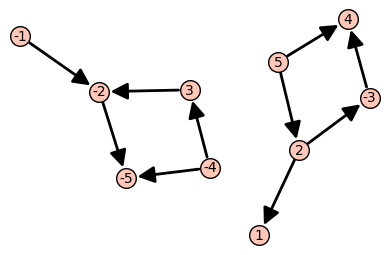
\includegraphics{g.png} \\
    Les variables $x_1,x_2,x_3,x_4$ et $x_5$ ansi que leurs négations sont représentées en sommets.
    Prenons maintenant la première clause. \\
    $(x_1 \lor \neg x_2)$ : on obtient donc les implications $\neg x_1 \Longrightarrow \neg x_2$ et $x_2 \Longrightarrow x_1$ \\
    Le processus est le même pour les autres clauses.
    \newpage
    \subsection{Algorithme (Exercice 4)}
    Voici une ébauche de la fonction formula\_2\_graph qui prend en argument un graphe et qui retourne son graphe associé.
    \subsubsection*{Le code}
    \begin{lstlisting}
        [...] #O(n^2)
        g = DiGraph()
        for var in clause: #O(n)
            g.add_vertices([int(var[0]), int(var[1])])
        sommets = g.vertices()
        for sommet in sommets:
            g.add_vertices([sommet*-1]) #O(n)
        [...]
        for i in range(0, len(clause)): #O(n)
            clause[i] = [int(clause[i][0]), int(clause[i][1])] #O(n)
        for var in clause: #O(n)
            g.add_edges([(var[0]*-1, var[1])])
            g.add_edges([(var[1]*-1, var[0])])
        return g
    \end{lstlisting} 
    Complexité : O($n^2$)\footnote{La fonction variables\_par\_classe est appelé}
    \subsubsection*{Explication}
    Le tableau clause contenant la liste des variables par clauses est obtenu de la même façon que l'exerice précédent.
    Nous allons ajouter chaque sommets au graphes. Tous d'abord nous allons prendres toutes les variables par clause. A chaque parcours de clause les deux variables sont rajoutées au graphes. \\
    \\ A ce moment là, le graphe n'est pas complet nous allons donc rajouter toutes les négations manquantes. On va donc stocker tous les sommets dans un tableau sommets. \\
    En implémentant les formules avec l'utilisation de "-" pour les négations ils nous aient facile de manipuler cette dernière. \\
    En effet, on va parcourir chaque sommet et rajouter sa négation en multipliant par -1\footnote{Il existait des variables qui avaient déjà leurs négations représentées sur le graphe. Cela n'est pas dérengant, les variables ont été écraser par elle-même.}. Les variables étant castées en entier précédement. \\
    \\
    Ensuite, nous allons rajouter les arrêtes. \\
    \\ Pour cela nous allons nous intéresser aux clauses contenant un couple de variables. Ces dernières étant stockées en chaine de caractères nous les avons castées en entier pour pouvoir les manipuler. \\
    Après cela nous pouvons effectuer les deux opérations pour rajouter les arrêtes. \\
    On parcours les différentes variables de chaque clause. On rajoute une arrête allant de la négation de la première variable jusqu'à la seconde variable. \\
    Ensuite on ajoute l'autre arrête entre la négation de la seconde variable et la première variable. \\
    On va ainsi rajouter 2 arrêtes par clauses.
    \section{Validitée d'une formule}
    \subsection{Théorie}
    Pour vérifié de la validitée d'une formule, nous allons analyser son graphe générer précédément. En applicant l'algorithme de Tarjan on obitent un ordre topologique sur les composantes fortement connexe. Soit $CC=[x_1,x_2,...,x_n]$ la liste des composantes connexes par tri topologique. \\
    Nous avons donc $\neg{(CC)}=[\neg x_1,\neg x_2,...,\neg x_n]$ qui est également une liste de composantes connexes. La formule est valide si la négation d'une variable n'est pas déjà présente. En considérent les composantes dans l’ordre inverse, on va
    leur affecter des valuations : tant qu’il reste une composante non valuée $CC$, on affecte à tous ses noeuds la valeur True et à tous les noeuds de $\neg CC$ la valeur False. 
    \subsection{Algorithme (Exercice 5)}
    Voici le code de la fonction est\_valide : 
    \subsubsection*{Le code}
    \begin{lstlisting}
        def est_valide(g):
            temp=list(strongly_connected_components_digraph(g))
            # Tarjan O(n)
            liste_connex = temp
            for connex in liste_connex: #O(n)
                tab = []
                for variable in connex: #O(n)
                    variable_temp = variable*-1
                    if tab.__contains__(variable_temp): #O(n)
                        return False
                tab.append(variable) #O(1)
        return True
    \end{lstlisting} 
    Complexité : O($n^3$)\footnote{La fonction sage : strongly\_connected\_components\_digraph() applique l'algorithme de Tarjan qui se fait en temps linéaire }
    \newpage
    \subsubsection*{Explication\footnote{Nous avons pas réussie à implémenter l'affectation}}
    Nous avons casté l'objet sage de type digraphe\footnote{Composantes fortements connexes} en liste pour pouvoir la manipuler. Ensuite nous allons pour chaque composantes connexes mettre dans un tableau une variable et vérifié si sa négation n'est pas déjà stockée, si elle l'est on retourne False si non on peut réinitialiser le tableau et passer à la prochaine composante fortement connexe. 
\end{document}
